\begin{activite}[Supprimer des parenthèses]

\begin{partie}[Un signe « + » devant des parenthèses]
\begin{enumerate}
\item Complète : $4x + (3 -7x) =  4x + \left((+ ...) + (-...)\right)$.

Écris alors cette expression sans parenthèse puis rédige une règle pour ajouter une somme algébrique. Que peut-on dire de parenthèses précédées d'un signe + ?
\item Écris l'expression suivante sans parenthèse : $G = 5 + (-6x + 1)$.
\end{enumerate}
\end{partie}

\begin{partie}[Un signe « $-$ » devant des parenthèses]
\begin{enumerate}
\item Quel est l'opposé de 5 ? Et celui de $-6,5$ ? Que vaut la somme de deux nombres opposés ? Que peut-on dire de deux nombres dont la somme est égale à 0 ?
\item Complète :
    \subitem $-3 + ... = 0$ donc l'opposé de $-3$ est ... ;
    \subitem $-3x^2 + ... = 0$ donc l'opposé de $-3x^2$ est ... ;
    \subitem $... + 5 = 0$ donc l'opposé de 5 est ... ;
    \subitem $3 + x + ... = 0$ donc l'opposé de $3 + x$ est ... ;
    \subitem $-x + ... = 0$ donc l'opposé de $-x$ est ... ;
    \subitem $-2x + 1 + ... = 0$ donc l'opposé de $-2x + 1$ est ... ;
    \subitem $... + 2x = 0$ donc l'opposé de $2x$ est ... ;
    \subitem $2 -x^2 + ... = 0$ donc l'opposé de $2 -x^2$ est ... .
\item Rappel : $a-b = a + \text{ opposé de } b$.

Complète : $F = 2x -(3 + x) = 2x + (...)$.

Déduis-en l'expression de F sans parenthèse.

\item De la même façon, écris sans parenthèse $G = 4 -(2 -x^2)$ et $H = 2x + 3 -(-2x + 1)$.

Rédige une règle pour soustraire une somme algébrique.
\end{enumerate}       
\end{partie}

\end{activite}



\begin{activite}[Écrire une expression littérale]

Avec des petits carrés identiques, disposés comme le montrent les figures ci-dessous, on constitue un nouveau carré.

\begin{center}
    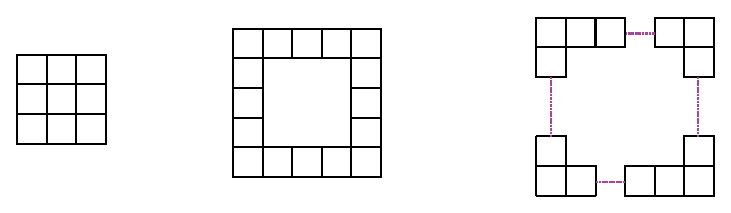
\includegraphics[width=.8\linewidth]{CLacti1}
\end{center}

\begin{enumerate}
\item Réalise une figure avec quatre petits carrés sur un côté. Indique le nombre total de carrés coloriés.

Recommence avec une figure de six petits carrés de côté.

S'il y a 100 petits carrés sur le côté, combien y-a-t-il de carrés coloriés au total ?
\item On appelle $n$ le nombre de petits carrés d'un côté. On veut obtenir une formule en fonction de n qui donne le nombre total de carrés coloriés dans le nouveau carré.
    \begin{enumerate}
        \item Chloé dit : « Je pense que la formule est $4n$ ! ».
        
        Sofiane lui répond alors : « Mais non ! Tu en as trop ! ».

        Justifie la réponse de Sofiane et établis une première formule.
        
        \item Sur les cahiers de trois élèves, on observe les schémas suivants :
        
        \begin{center}
        Schéma de Jean \hfill Schéma de Fatima \hfill Schéma de Bakari
            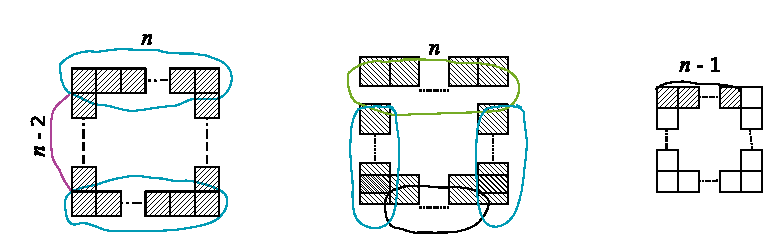
\includegraphics[width=.8\linewidth]{CLacti2}
        \end{center}

        En suivant les découpages de Jean et de Fatima, établis deux nouvelles formules.
        
        À l'aide de son schéma, Bakari remarque que le nombre de carrés coloriés est un multiple de 4.
        
        Justifie sa remarque et déduis-en une quatrième formule.
        
        \item En utilisant chacune de ces quatre formules, calcule le nombre total de carrés coloriés lorsqu'il y en a 15 sur un côté. Les résultats trouvés étaient-ils prévisibles ?
    \end{enumerate}
\end{enumerate}
\end{activite}



\begin{activite}[Conjecturer, démontrer]

On considère le programme de calculs suivant :

\begin{center}
    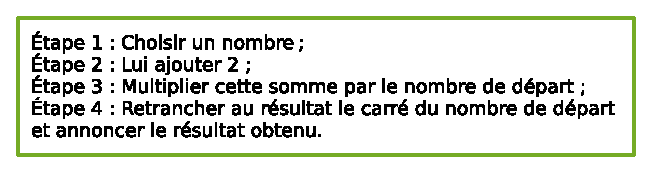
\includegraphics[width=.6\linewidth]{CLacti3}
\end{center}

\begin{enumerate}

\item Effectue le programme en choisissant 5 comme nombre de départ puis $-8$ et enfin $3,45$. Quelle remarque peux-tu faire ?
\item\label{CLact1} Dans un tableur, reproduis le tableau ci-dessous.

\begin{center}
    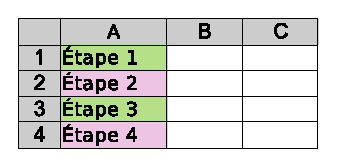
\includegraphics[width=.3\linewidth]{CLacti4}
\end{center}

Complète la première ligne avec les nombres entiers de 1 à 10 puis programme les cellules pour qu'elles affichent les résultats pour chaque étape du programme de calculs. Que remarques-tu ?
\item\label{CLact2} Remplace les nombres de la première ligne par des nombres entiers négatifs puis par des nombres décimaux relatifs. Que remarques-tu ?
\item On appelle $x$ le nombre de départ. Écris les étapes en fonction de $x$ et retrouve alors ce que tu as remarqué aux questions \ref{CLact1} et \ref{CLact2}.
\end{enumerate}
\end{activite}



\begin{activite}[L'art du contre-exemple]

\begin{enumerate}
\item Calcule $x^2 + 3$ puis $3x + 1$ en remplaçant d'abord $x$ par 1 puis par 2. Que remarques-tu ? Est-ce que  $x^2 + 3 = 3x + 1$ ? Justifie.
\item En étudiant un cube, Zoé remarque qu'il possède $F = 6$ faces et $S = 8$ sommets. Elle écrit $F + 2 = S$. Cette formule est-elle vraie pour un parallélépipède ? Est-elle vraie pour la pyramide ci-dessous ?

\begin{center}
    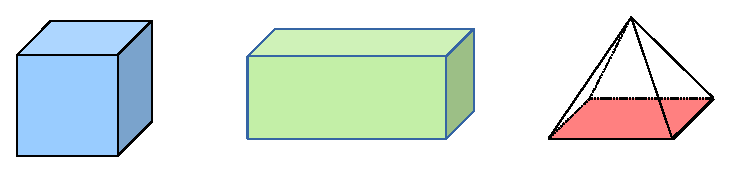
\includegraphics[width=.8\linewidth]{CLacti5}
\end{center}

\end{enumerate}
\end{activite}



\begin{activite}[Rectangles cousins]

\begin{enumerate}
\item Calcule le périmètre et l'aire des deux rectangles suivants. Que remarques-tu ?

\begin{center}
    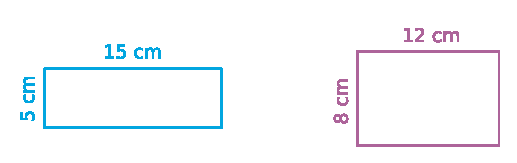
\includegraphics[width=.6\linewidth]{CLacti6}
\end{center}

Dans cette activité, on s'intéresse uniquement aux rectangles dont le périmètre est 40\,cm.

\item Un 3\up{e} rectangle a pour longueur $L = 16,5$\,cm. Calcule sa largeur $\ell$ puis son aire. 

\begin{center}
    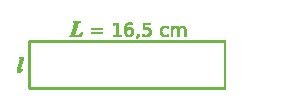
\includegraphics[width=.3\linewidth]{CLacti7}
\end{center}

\item Donne les mesures d'un 4\up{e} rectangle de même périmètre.
\item La longueur peut-elle valoir 8\,cm ? Et 21\,cm ? Justifie et donne les valeurs possibles pour la longueur.
\item Écris une expression qui permet de calculer la largeur $\ell$ en fonction de la longueur $L$. 
\item En voulant exprimer l'aire $\mathcal{A}$ du rectangle en fonction de sa longueur $L$, des élèves ont donné les réponses suivantes.
    \subitem Gaël	: $\mathcal{A} = L \times 20 - L$
	\subitem Inès	: $\mathcal{A} = 2 \times L + 2 \times (20 - L)$
	\subitem Hamid	: $\mathcal{A} = L \times (20 - L)$
	\subitem José	: $\mathcal{A} = L \times 20 - 2 \times L$
	\subitem Karen	: $\mathcal{A} = 20 L - L^2$
	\subitem Liam	: $\mathcal{A} = L^2 - 20 \times L$

Parmi ces expressions, lesquelles sont fausses ? Y a-t-il plusieurs bonnes réponses ? Justifie.

\item À l'aide d'un tableur, calcule l'aire de ces rectangles pour toutes les valeurs entières de $L$ possibles. 
\item Pour quelle valeur de $L$ l'aire semble-t-elle la plus grande ?
\end{enumerate}
\end{activite}

 



                                          


